\chapter{OpenBTS}

OpenBTS is a software implementation of a GSM access point \cite{wikiOpenBTS}.
It allows common GSM-compatible mobile phones to be used a SIP endpoints to VoIP-based
networks. It implements the lower three layers of the industry-standard GSM
protocol stack. OpenBTS is an open source software written in C++. Some 
additional real-time components of it are written in Erlang.

OpenBTS was first developed with a goal to provide low-cost and easily 
deployable GSM networks in poor and rural ureas.

\section{GSM architecture of OpenBTS}
In an OpenBTS based network, the layers of conventional GSM network above layer 3
are replaced by OpenBTS itself. The functions of the BSC are handled internally.
The call handling functionalities of the MSC are handed over to a VoIP 
softswitch or PBX like Asterisk. In fact, multiple OpenBTS networks 
can be set up sharing a common VoIP softswitch or PBX \cite{wikiOpenBTS}.

The GSM-based Um interface of OpenBTS 
does not use any standard GSM hardware. Instead OpenBTS uses software-defined
radio transceivers for its Um interface. The USRP from Ettus Research was the
first such hardware device to be used for OpenBTS Um interface \cite{wikiOpenBTS}.



\section{The OpenBTS Application Suite}
The OpenBTS Application Suite comes with several software applications that 
are listed as follows:

\begin{itemize}
\item \textbf{OpenBTS}
\item \textbf{Transceiver}
\item \textbf{SMQueue}
\item \textbf{Asterisk}
\item \textbf{SIPAuthServe}
\end{itemize}

Besides these, there are optional services supported through 
external servers and interfaced to OpenBTS through various protocols. For 
example, the RRLP server.

\subsection{OpenBTS}
The OpenBTS application contains various functions beginning from Layer 1 upto
Layer 3/Layer 4. The Layer 1 functions are:
\begin{itemize}
\item TDM functions
\item FEC functions
\item closed loop power and timing controls
\end{itemize}

\emph{LAPDm} is the only Layer 2 function implemented in the OpenBTS 
application.

The Layer 3 functions are:
\begin{itemize}
\item radio resource management
\item mobility management
\item call control
\end{itemize}

\emph{GSM-SIP gateway for text messaging} is the Layer 4 function included
in OpenBTS.

OpenBTS itself does not contain any speech transcoding
functions above the L1 FEC parts.


\subsection{Transceiver}
The transceiver application performs the radiomodem functions of GSM 05.05 and manages 
the Gigabit Ethernet interface
(USB2 interface, in case
of USRP1 or older models) to the radio hardware.

\subsection{SMQueue}
SMQueue is a store-and-forward server that is used for 
text messaging in the OpenBTS system. SMQueue is required to send 
a text message from one MS to another, or to an MS from any source.

\subsection{SIP router/PBX}

OpenBTS uses a SIP router or PBX to perform the 
call control functions that are normally performed by the MSC
in a conventional GSM network. These switches also provide transcoding 
services.

The SIP router used in OpenBTS is Asterisk by default. Though there are other
PBXs available in the market like Yate, FreeSwitch, etc.

\subsection{SIPAuthServe}
An application that implements Subscriber Registry, the database of subscriber 
information that replaces both the Asterisk SIP registry and the GSM Home 
Location Register (HLR) found in a conventional GSM network.

\section{Network organization}
In the simplest network, with just a single access point, all the applications run
on the same embedded computer as shown in figure~\ref{fig:btsSimple}.

In larger network, with more than one access points, one of them can behave as a master and provide servers to the rest of them.
Figure~\ref{fig:btsLarge} shows a network with two access points where
a master access points is providing servers to the other one.

The Transceiver applications and the OpenBTS must run in each GSM/SIP access point. 
The Asterisk and the Subscriber Registry applications (SIPAuthServe) 
communicate via the filesystem, so they must run in the same computer,
but that computer can be remote to the access point. 
SMQueue and other servers can run in any access point and can have 
multiple instances.
\begin{figure}
  \centering
    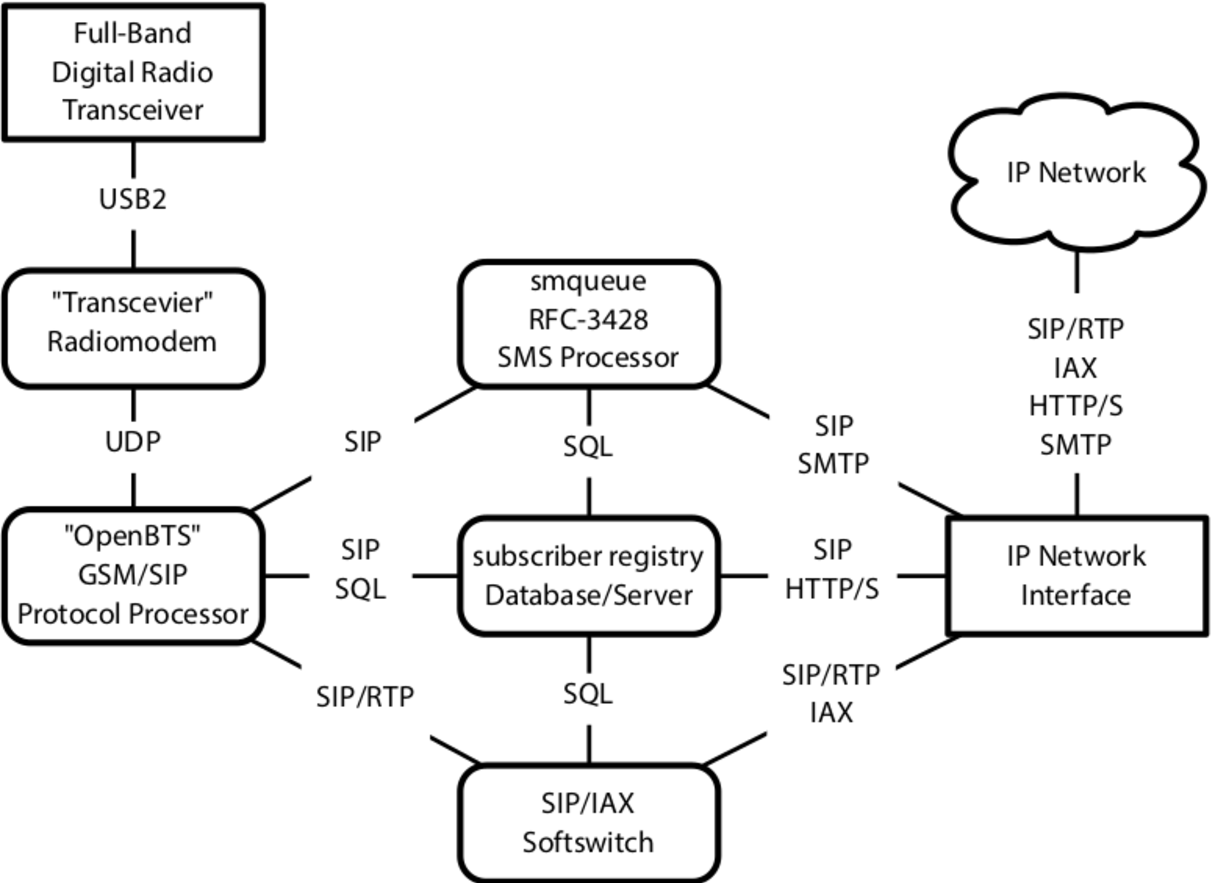
\includegraphics[width=\textwidth]{../images/btsSimple}
  \caption[Simplest OpenBTS network]{Components of the OpenBTS application suite 
  and their communication channels as installed in each
access point. Sharp-cornered boxes are hardware components.
Round-cornered boxes are software components \protect\cite{openbtsMan}.}
  \label{fig:btsSimple}
\end{figure}

\begin{figure}
  \centering
    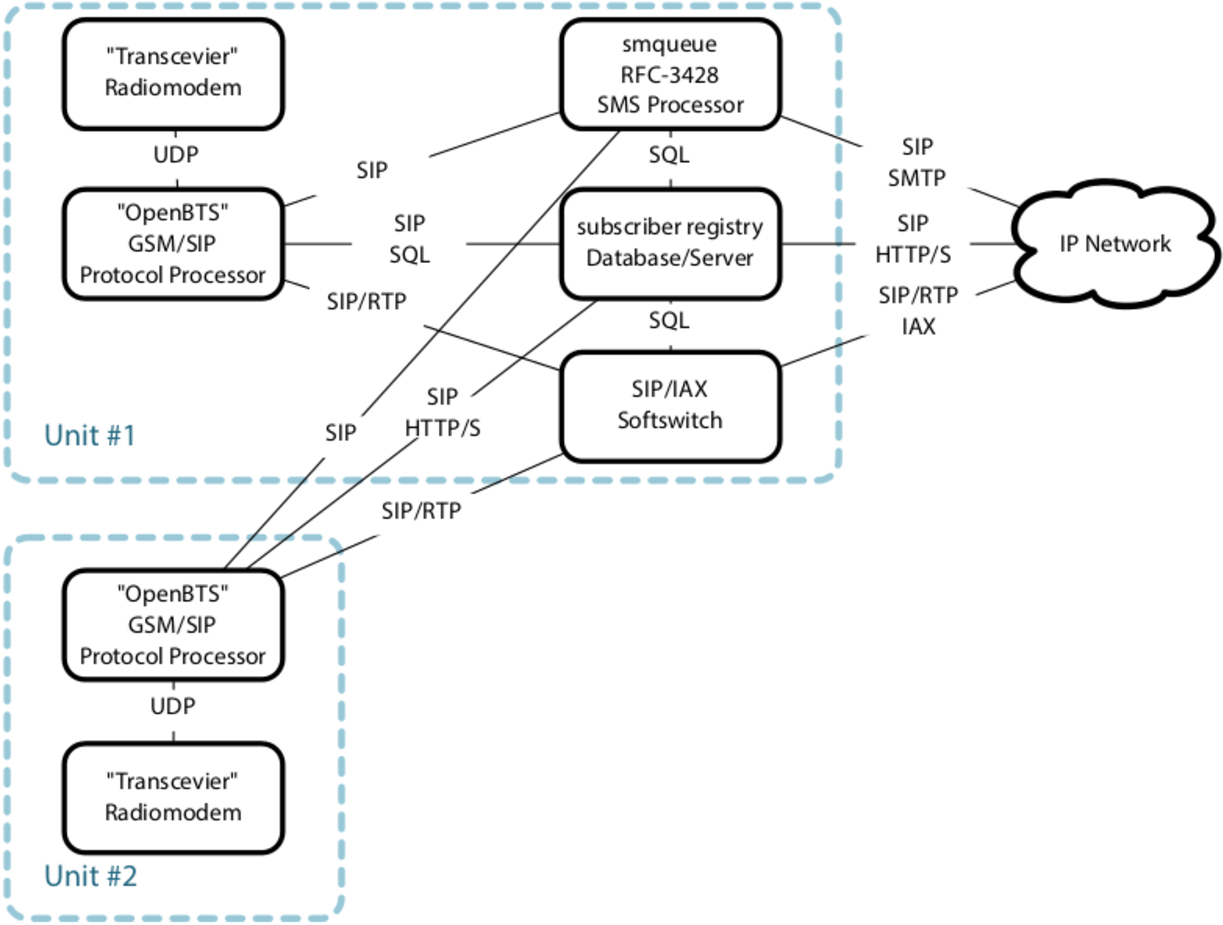
\includegraphics[width=\textwidth]{../images/btsLarge}
  \caption[OpenBTS network with two access points]{Two access points with unit 
  \#1 providing servers for both \protect\cite{openbtsMan}}
  \label{fig:btsLarge}
\end{figure}
